%TODO: provide your details here.

\begin{frame}
    \frametitle{About Your Fellows}
    \begin{itemize}
        \item Hi there! We are \textcolor{red}{\textbf{Abuhurairah}} {and }\textcolor{red}{\textbf{Talha}}.
        \item We are Associate Students at ITU.
    \end{itemize}
\end{frame}

\begin{frame}
    \frametitle{\textbf{Secretary Problem}}
        \item\textcolor{black}{Goal:}
       \vspace{0.3cm}
        \begin{itemize}
            \item Select the best secretary (or candidate) out of n applicants.
        \end{itemize}
\end{frame}

\begin{frame}
    \frametitle{Secretary Problem Diagram}
    \begin{center}
    \begin{tikzpicture}[scale=1.0, >=Stealth]

        \draw (0,0) rectangle (8,1);

        \fill[silver!11] (0,0) rectangle (3,1);

        \fill[green!20] (3,0) rectangle (8,1);

        \draw (0,0) rectangle (8,1);

        \draw[<->,thick] (0,1.2) -- node[above]{\(\displaystyle k\)} (3,1.2);

        \draw[<->,thick] (3,1.2) -- node[above, xshift=20pt]{\(\displaystyle n - k\)} (8,1.2);

        \node[above] at (1.5,0.2) {\textcolor{black}{\(x\) (Best in \(k\))}};

        \draw[dashed] (5,0) -- (5,1.4);
        \node[above] at (5,1.4){\(\displaystyle i\)};

    \end{tikzpicture}
    \end{center}
\end{frame}

\begin{frame}
    \frametitle{Secretary Problem Diagram}
    \begin{center}
    \begin{tikzpicture}[scale=1.0, >=Stealth]

        \draw (0,0) rectangle (8,1);

        \fill[silver!11] (0,0) rectangle (3,1);

        \fill[green!20] (3,0) rectangle (8,1);

        \draw (0,0) rectangle (8,1);

        \draw[<->,thick] (0,1.2) -- node[above]{\(\displaystyle k\)} (3,1.2);

        \draw[<->,thick] (3,1.2) -- node[above, xshift=20pt]{\(\displaystyle n - k\)} (8,1.2);

        \node[above] at (1.5,0.2) {\textcolor{black}{\(x\) (Best in \(k\))}};

        \draw[dashed] (5,0) -- (5,1.4);
        \node[above] at (5,1.4){\(\displaystyle i\)};

        \node[align=center] at (4,-0.6) {\small Dashed line marks candidate \(i\):\\the first candidate in the decision phase \\ whose score exceeds \(x\).};

    \end{tikzpicture}
    \end{center}
\end{frame}

\begin{frame}
    \frametitle{Recap: \textbf{Secretary Problem}}
    \begin{itemize}
        \item \textbf{Secretary Problem}: Select the best candidate out of \(n\) applicants.
        \item Strategy: \begin{itemize}
            \item Interview the first \(k\) candidates (skip them).
            \item Let \(x\) be the best candidate among the first \(k\).
            \item For any candidate \(i\) (with \(i > k\)), if \(score(i) > score(x)\) then consider hiring.
        \end{itemize}
    \end{itemize}
\end{frame}

\begin{frame}
    \frametitle{Probability of Hiring the Best Candidate}
    \begin{itemize}
        \item We wish to compute:
        \[
        P(\text{Hiring best candidate}) = \sum_{i=1}^{n} \Pr(i\text{ is best}) \times \Pr(\text{hire } i \mid i\text{ is best})
        \]
        \item Since every candidate is equally likely to be the best:
        \[
        \Pr(i\text{ is best}) = \frac{1}{n}.
        \]
    \end{itemize}
\end{frame}

\begin{frame}
    \frametitle{Conditional Probability}
    \begin{itemize}
        \item The probability of hiring candidate \(i\) given that \(i\) is best is:
        \[
        \Pr(\text{hire } i \mid i\text{ is best}) = \Pr\Big(\text{no candidate before } i \text{ is hired}\Big)
        \]
        \item This probability is modeled as:
        \[
        \frac{k-1}{i-1}.
        \]
        \item Thus, we have:
        \[
        P(\text{Hiring best candidate}) = \frac{k-1}{n} \sum_{i=k+1}^{n} \frac{1}{i-1}.
        \]
    \end{itemize}
\end{frame}

\begin{frame}
    \frametitle{Harmonic Series Approximation}
    \begin{itemize}
        \item Recognize that:
        \[
        \sum_{i=k+1}^{n} \frac{1}{i-1} = \sum_{j=k}^{n-1} \frac{1}{j} \quad \text{(with } j=i-1\text{)}
        \]
        \item The harmonic series \(H_m = \sum_{i=1}^{m} \frac{1}{i}\) is approximately:
        \[
        H_m \approx \ln(m) \quad \text{(or } \ln(m+1)\text{)}.
        \]
        \item Therefore:
        \[
        P(\text{Hiring best candidate}) \approx \frac{k-1}{n}\left[\ln(n-1)-\ln(k-1)\right].
        \]
    \end{itemize}
\end{frame}

\begin{frame}
    \frametitle{Optimizing the Success Probability}
    \begin{itemize}
        \item Let \(j = k-1\). Then:
        \[
        P(\text{success}) = \frac{j}{n}\left[\ln(n-1)-\ln(j)\right].
        \]
        \item To maximize \(P(\text{success})\), we differentiate with respect to \(j\) and set the derivative to zero.
    \end{itemize}
\end{frame}

\begin{frame}
    \frametitle{Derivative Calculation}
    \begin{itemize}
        \item Define:
        \[
        u = \frac{j}{n} \quad \text{and} \quad v = \ln(n-1)-\ln(j).
        \]
        \item Then:
        \[
        \frac{du}{dj} = \frac{1}{n} \quad \text{and} \quad \frac{dv}{dj} = -\frac{1}{j}.
        \]
        \item Applying the product rule:
        \[
        \frac{d}{dj}(uv) = u\frac{dv}{dj} + v\frac{du}{dj} 
        = \frac{j}{n}\left(-\frac{1}{j}\right) + \frac{1}{n}\left[\ln(n-1)-\ln(j)\right].
        \]
        \item Simplifying:
        \[
        \frac{d}{dj}(uv) = -\frac{1}{n} + \frac{1}{n}\left[\ln(n-1)-\ln(j)\right].
        \]
    \end{itemize}
\end{frame}

\begin{frame}
    \frametitle{Setting the Derivative to Zero}
    \begin{itemize}
        \item Set:
        \[
        \frac{1}{n}\Big[\ln(n-1)-\ln(j)-1\Big] = 0.
        \]
        \item This implies:
        \[
        \ln(n-1)-\ln(j)-1 = 0 \quad \rightarrow \quad \ln(j)=\ln(n-1)-1.
        \]
        \item Exponentiating both sides:
        \[
        j = \frac{n-1}{e}.
        \]
    \end{itemize}
\end{frame}

\begin{frame}
    \frametitle{Final Result}
    \begin{itemize}
        \item Recall that \(j = k-1\). Thus:
        \[
        k = \frac{n-1}{e} + 1.
        \]
        \item For large \(n\), this simplifies to:
        \[
        k \approx \frac{n}{e}.
        \]
        \item \textbf{Optimal Strategy:} Skip the first \(\frac{n}{e}\) candidates.
    \end{itemize}
\end{frame}

% Slide: Inroduction to Heap
\begin{frame}
    \begin{center}
        \vspace*{1cm}  % Add some vertical space at the top
        {\Large \textcolor{red}{\textbf{Algorithms, Design \& Analysis}}}
        
        \vspace{0.5cm}  % Space between title and subtitle
        \textcolor{blue}{\textbf{Introduction to Heap}}
        
        \vspace{1cm}  % Space below subtitle
    \end{center}
\end{frame}

% Slide: Introduction to Heap
\begin{frame}{What is a Heap?}
    \begin{itemize}
        \item A complete binary tree.
    \end{itemize}

\end{frame}

% Slide: Complete Binary tree

\begin{frame}{What is a Complete Binary Tree?}
\textbf{Definition:}
\begin{itemize}
    \item A binary tree where all levels are completely filled, except possibly the last one.
    \item The last level must be filled from left to right.
\end{itemize}
\textbf{Example of a Complete Binary Tree:}

\begin{center}

 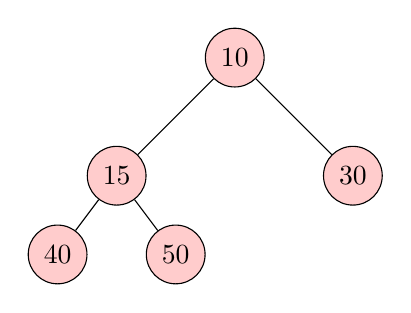
\begin{tikzpicture}[every node/.style={circle,draw,fill=red!20}]
    \node {10}
        child [level distance=1.5cm, sibling distance=3cm] { 
            node {15} 
            child [level distance=1cm, sibling distance=1.5cm] { node {40} } 
            child [level distance=1cm, sibling distance=1.5cm] { node {50} } 
        }
        child [level distance=1.5cm, sibling distance=3cm] { 
            node {30} 
           % child [level distance=1cm, sibling distance=1.5cm] { node {99} } 
           % child [level distance=1cm, sibling distance=1.5cm] { node {40} } 
        };
   \end{tikzpicture}
\end{center}
\end{frame}

% Slide: Height of a Complete Binary Tree - Introduction
\begin{frame}{Height of a Complete Binary Tree}
    \begin{itemize}
        \item In a complete binary tree with \( n \) nodes:
        \begin{itemize}
            \item The height \( h \) is approximately \( \log_2 n \).
            \item More precisely, \( h = \lfloor \log_2 n \rfloor \).
        \end{itemize}
    \end{itemize}
    \pause
    \centering
    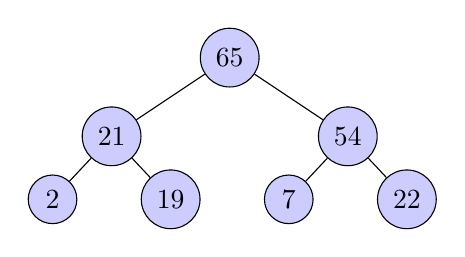
\begin{tikzpicture}[every node/.style={circle,draw,fill=blue!20}]
        \node {65}
            child [level distance=1cm, sibling distance=3cm] { 
                node {21} 
                child [level distance=0.8cm, sibling distance=1.5cm] { node {2} } 
                child [level distance=0.8cm, sibling distance=1.5cm] { node {19} } 
            }
            child [level distance=1cm, sibling distance=3cm] { 
                node {54} 
                 child [level distance=0.8cm, sibling distance=1.5cm] { node {7} } 
                child [level distance=0.8cm, sibling distance=1.5cm] { node {22} } 
            };
    \end{tikzpicture}
\end{frame}

% Slide: Mathematical Derivation
\begin{frame}{Mathematical Derivation of Height}
    \begin{itemize}
        \item A complete binary tree follows the pattern:
        \begin{equation}
            n = 1 + 2 + 4 + \dots + 2^h
        \end{equation}
        \item Using the summation formula for a geometric series:
        \begin{equation}
            n = \sum_{i=0}^{h} 2^i = 2^{h+1} - 1
        \end{equation}
        \item Solving for height by taking logarithms:
        \begin{equation}
            h = \lfloor \log_2(n + 1) - 1 \rfloor
        \end{equation}
    \end{itemize}
\end{frame}

% Slide: Summation Formula & Node Count
\begin{frame}{Summation and Node Count}
    \begin{itemize}
        \item The number of nodes at level \( i \) in a complete binary tree is \( 2^i \).
        \item The total number of nodes in a complete binary tree:
        \begin{equation}
            n = \sum_{i=0}^{h} 2^i = 2^{h+1} - 1
        \end{equation}
        \item Rearranging for height:
        \begin{equation}
            h = \lfloor \log_2 n \rfloor
        \end{equation}
    \end{itemize}
    \centering
   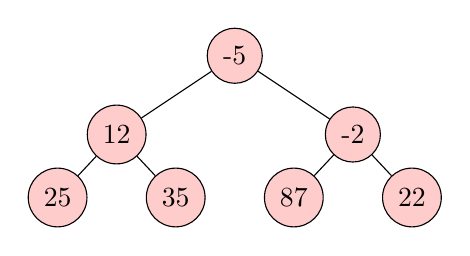
\begin{tikzpicture}[every node/.style={circle,draw,fill=red!20}]
        \node {-5}
            child [level distance=1cm, sibling distance=3cm] { 
                node {12} 
                child [level distance=0.8cm, sibling distance=1.5cm] { node {25} } 
                child [level distance=0.8cm, sibling distance=1.5cm] { node {35} } 
            }
            child [level distance=1cm, sibling distance=3cm] { 
                node {-2} 
                 child [level distance=0.8cm, sibling distance=1.5cm] { node {87} } 
                child [level distance=0.8cm, sibling distance=1.5cm] { node {22} } 
            };
    \end{tikzpicture}
\end{frame}

% Slide: Final Height Formula & Conclusion
\begin{frame}{Final Height Formula and Conclusion}
    \begin{itemize}
        \item We derived that the height of a complete binary tree is:
        \begin{equation}
            h = \lfloor \log_2 n \rfloor
        \end{equation}
        \item Since heaps are complete binary trees, their height follows this formula.
       % \item This is useful in analyzing heap operations like insertion, deletion, and heapify, which run in \( O(\log n) \) time.
    \end{itemize}
\end{frame}

% Slide: Example to Verify Formulas
\begin{frame}{Example: Verifying Height Formula}
    \begin{itemize}
        \item Consider a complete binary tree with \( \textbf{n = 14} \) nodes.
        \item Using our formula:
        \begin{equation}
            h = \lfloor \log_2 14 \rfloor = 3
        \end{equation}
        \item Visualizing the tree:
    \end{itemize}
    \centering
  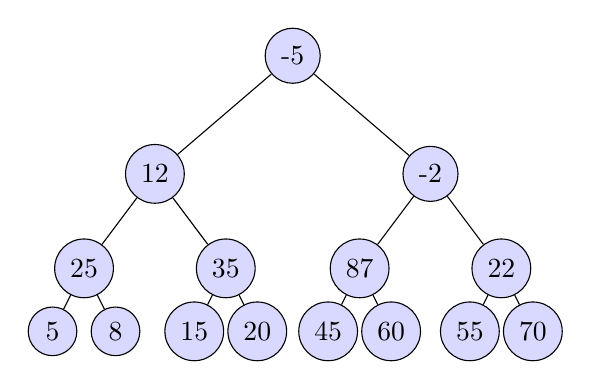
\begin{tikzpicture}[every node/.style={circle,draw,fill=blue!15}]
        \node {-5}
            child[level distance=1.5cm, sibling distance=3.5cm]  { 
                node {12} 
                child [level distance=1.2cm, sibling distance=1.8cm] { 
                    node {25} 
                    child [level distance=0.8cm, sibling distance=0.8cm] { node {5} } 
                    child [level distance=0.8cm, sibling distance=0.8cm] { node {8} }
                }
                child [level distance=1.2cm, sibling distance=1.8cm] { 
                    node {35} 
                    child [level distance=0.8cm, sibling distance=0.8cm] { node {15} }
                    child [level distance=0.8cm, sibling distance=0.8cm] { node {20} }
                }
            }
            child[level distance=1.5cm, sibling distance=3.5cm]  { 
                node {-2} 
                child [level distance=1.2cm, sibling distance=1.8cm] { 
                    node {87} 
                    child [level distance=0.8cm, sibling distance=0.8cm] { node {45} }
                    child [level distance=0.8cm, sibling distance=0.8cm] { node {60} }
                }
                child  [level distance=1.2cm, sibling distance=1.8cm]{ 
                    node {22} 
                    child [level distance=0.8cm, sibling distance=0.8cm]{ node {55} }
                    child[level distance=0.8cm, sibling distance=0.8cm] { node {70} }
                }
            };
    \end{tikzpicture}
    \pause
    \begin{itemize}
        \item As observed, the tree has exactly \( \textbf{h = 3} \) levels, confirming our formula.
    \end{itemize}
\end{frame}


% Slide: Introduction to Heap
\begin{frame}{What is a Heap?}
    \begin{itemize}
        \item A complete binary tree.
        \item Heap property:
        \begin{itemize}
            \item \textcolor{blue}{Max Heap}: Parent node \(\geq\) children.
            \item \textcolor{red}{Min Heap}: Parent node \(\leq\) children.
        \end{itemize}
    \end{itemize}
    \textbf{Example of a Min Heap:}
    
    \centering
   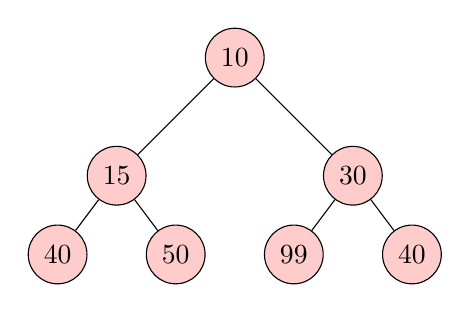
\begin{tikzpicture}[every node/.style={circle,draw,fill=red!20}]
    \node {10}
        child [level distance=1.5cm, sibling distance=3cm] { 
            node {15} 
            child [level distance=1cm, sibling distance=1.5cm] { node {40} } 
            child [level distance=1cm, sibling distance=1.5cm] { node {50} } 
        }
        child [level distance=1.5cm, sibling distance=3cm] { 
            node {30} 
            child [level distance=1cm, sibling distance=1.5cm] { node {99} } 
            child [level distance=1cm, sibling distance=1.5cm] { node {40} } 
        };
   \end{tikzpicture}
\end{frame}   


% Slide: Examples of Min Heap
\begin{frame}{Examples of Min Heap}
    \centering
    \textbf{Example 1:} \\
    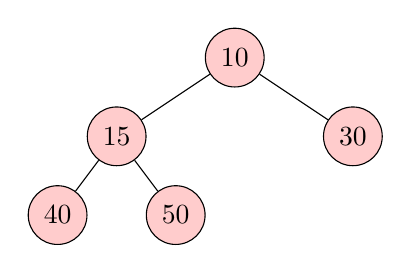
\begin{tikzpicture}[every node/.style={circle,draw,fill=red!20}]
        \node {10}
            child [level distance=1cm, sibling distance=3cm] { 
                node {15} 
                child [level distance=1cm, sibling distance=1.5cm] { node {40} } 
                child [level distance=1cm, sibling distance=1.5cm] { node {50} } 
            }
            child [level distance=1cm, sibling distance=3cm] { 
                node {30} 
            };
    \end{tikzpicture}
    
    \vspace{0.3cm} % Space between examples

    \textbf{Example 2:} \\
    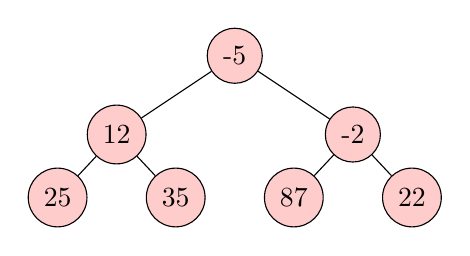
\begin{tikzpicture}[every node/.style={circle,draw,fill=red!20}]
        \node {-5}
            child [level distance=1cm, sibling distance=3cm] { 
                node {12} 
                child [level distance=0.8cm, sibling distance=1.5cm] { node {25} } 
                child [level distance=0.8cm, sibling distance=1.5cm] { node {35} } 
            }
            child [level distance=1cm, sibling distance=3cm] { 
                node {-2} 
                 child [level distance=0.8cm, sibling distance=1.5cm] { node {87} } 
                child [level distance=0.8cm, sibling distance=1.5cm] { node {22} } 
            };
    \end{tikzpicture}
\end{frame}

% Slide: Examples of Max Heap
\begin{frame}{Examples of Max Heap}
    \centering
    \textbf{Example 1:} \\
    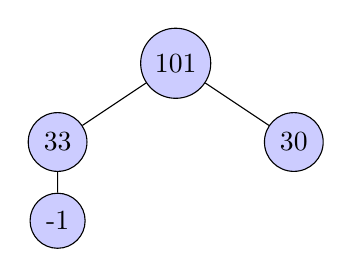
\begin{tikzpicture}[every node/.style={circle,draw,fill=blue!20}]
        \node {101}
            child [level distance=1cm, sibling distance=3cm] { 
                node {33} 
                child [level distance=1cm, sibling distance=1.5cm] { node {-1} } 
            }
            child [level distance=1cm, sibling distance=3cm] { 
                node {30} 
            };
    \end{tikzpicture}
    
    \vspace{0.3cm} % Space between examples

    \textbf{Example 2:} \\
    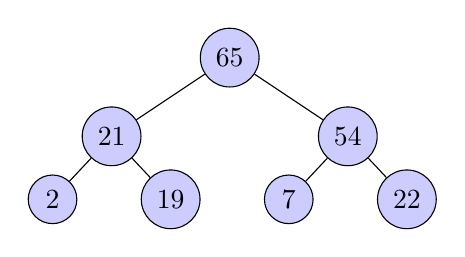
\begin{tikzpicture}[every node/.style={circle,draw,fill=blue!20}]
        \node {65}
            child [level distance=1cm, sibling distance=3cm] { 
                node {21} 
                child [level distance=0.8cm, sibling distance=1.5cm] { node {2} } 
                child [level distance=0.8cm, sibling distance=1.5cm] { node {19} } 
            }
            child [level distance=1cm, sibling distance=3cm] { 
                node {54} 
                 child [level distance=0.8cm, sibling distance=1.5cm] { node {7} } 
                child [level distance=0.8cm, sibling distance=1.5cm] { node {22} } 
            };
    \end{tikzpicture}
\end{frame}

\begin{frame}{Accessing a Parent Node in a Heap}
    \textbf{Formula:}
    \begin{itemize}
        \item In a zero-based index heap stored as an array:
        \[
        \text{Parent}(i) = \frac{i-1}{2} \quad \text{(using integer division)}
        \]
        \item This means that for any node at index \( i \), its parent is found at index \( \lfloor (i-1)/2 \rfloor \).
    \end{itemize}

    
\end{frame}

\begin{frame}{Accessing a Parent Node in a Heap}
      
    \textbf{Visualization:}
    \begin{center}
    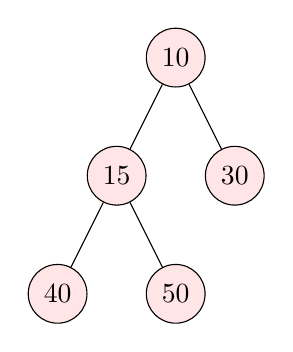
\begin{tikzpicture}[every node/.style={circle,draw,fill=red!10}]
        \node {10} % Root
            child { 
                node {15} % Left child
                child { node {40} } 
                child { node {50} } 
            }
            child { 
                node {30} % Right child
            };
    \end{tikzpicture}
    \end{center}

    %\vspace{0.2cm}
    
    \textbf{Example:}
    \begin{itemize}
        \item The node \( 40 \) is at the index \( 3 \).
        \item Using the formula: \(\lfloor (3-1)/2 \rfloor = 1 \), so its parent is at index \textbf{1} (value = \textbf{15}).
    \end{itemize}
\end{frame}

\begin{frame}{Accessing Child Nodes in a Heap}
    \textbf{Formulas:}
    \begin{itemize}
        \item In a zero-based index heap stored as an array:
        \[
        \text{Left Child}(i) = 2i + 1
        \]
        \[
        \text{Right Child}(i) = 2i + 2
        \]
        \item This means that for any node at index \( i \):
        \begin{itemize}
            \item The left child is found at index \( 2i + 1 \).
            \item The right child is found at index \( 2i + 2 \).
        \end{itemize}
    \end{itemize}

    \vspace{0.5cm}
    
\end{frame}

\begin{frame}{Accessing Child Nodes in a Heap}
       
    \textbf{Visualization:}
    \begin{center}
    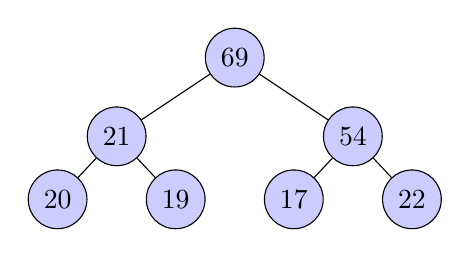
\begin{tikzpicture}[every node/.style={circle,draw,fill=blue!20}]
        \node {69}
            child [level distance=1cm, sibling distance=3cm] { 
                node {21} 
                child [level distance=0.8cm, sibling distance=1.5cm] { node {20} } 
                child [level distance=0.8cm, sibling distance=1.5cm] { node {19} } 
            }
            child [level distance=1cm, sibling distance=3cm] { 
                node {54} 
                 child [level distance=0.8cm, sibling distance=1.5cm] { node {17} } 
                child [level distance=0.8cm, sibling distance=1.5cm] { node {22} } 
            };
    \end{tikzpicture}
    \end{center}

    \vspace{0.2cm}
    
    \textbf{Example:}
    \begin{itemize}
        \item Node \( 54 \) is at index \( 2 \).
        \item Using the formulas:
        \begin{itemize}
            \item \textbf{Left Child}: \( 2(2) + 1 = 5 \) (value = \textbf{17}).
            \item \textbf{Right Child}: \( 2(2) + 2 = 6 \) (value = \textbf{22}).
        \end{itemize}
    \end{itemize}
\end{frame}


\begin{frame}{How Do We Build a Heap?  (Min Heap)}
\textbf{Steps to Build a Heap}
\begin{enumerate}
\item Start with an unsorted list of numbers.
\item Turn it into a tree shape.
\item Fix the tree by making sure each parent is smaller than its children.
\item Keep fixing until the smallest number is on top!
\end{enumerate}
\end{frame}

\begin{frame}{Understanding Heapify}
\textbf{What is Heapify?}
\begin{itemize}
\item Heapify is like cleaning up a messy room!
\item It makes sure each parent follows the heap rule.
\item If a child is bigger (in case of min-heap), we swap places.
\item We keep fixing from bottom to top.
\end{itemize}
\end{frame}

\begin{frame}{Let’s Build a Min-Heap!}
\textbf{Given Numbers:} {4, 10, 3, 5, 1, 7, 6, 8, 9}

\textbf{Step 1: Turn into a Tree}
\begin{center}
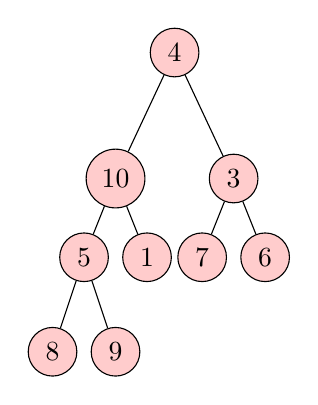
\begin{tikzpicture}[every node/.style={circle,draw,fill=red!20}]
\node {4}
child [level distance=1.6cm, sibling distance=1.5cm]  { node {10}
child[level distance=1cm, sibling distance=0.8cm] { node {5}
child[level distance=1.2cm, sibling distance=0.8cm] { node {8} }
child[level distance=1.2cm, sibling distance=0.8cm] { node {9} }}
child [level distance=1cm, sibling distance=0.8cm]{ node {1} }
}
child[level distance=1.6cm, sibling distance=1.5cm]  { node {3}
child[level distance=1cm, sibling distance=0.8cm] { node {7} }
child[level distance=1cm, sibling distance=0.8cm] { node {6} }
};
\end{tikzpicture}
\end{center}
\end{frame}

\begin{frame}{Apply Heapify Step-by-Step}
\textbf{Steps:}
\begin{enumerate}
\item Start from the last node.
\item Check if it's valid.
\item Swap if needed.
\item Repeat until the top is the smallest.
\end{enumerate}
\end{frame}
\begin{frame}{Step-by-Step Heapify Process}
\textbf{Starting from the last index, checking each node:}
\end{frame}

\begin{frame}{Step 1: Check Node 8 (Valid)}
\begin{center}
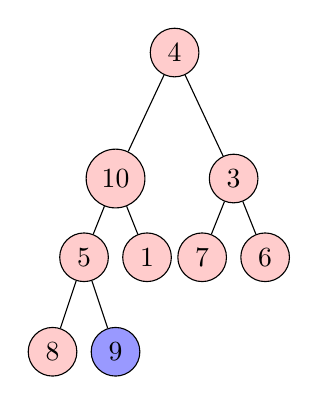
\begin{tikzpicture}[every node/.style={circle,draw,fill=red!20}]
\node {4}
child [level distance=1.6cm, sibling distance=1.5cm]  { node {10}
child[level distance=1cm, sibling distance=0.8cm] { node {5}
child[level distance=1.2cm, sibling distance=0.8cm] { node {8} }
child[level distance=1.2cm, sibling distance=0.8cm] { node[fill=blue!40] {9} }}
child [level distance=1cm, sibling distance=0.8cm]{ node {1} }
}
child[level distance=1.6cm, sibling distance=1.5cm]  { node {3}
child[level distance=1cm, sibling distance=0.8cm] { node {7} }
child[level distance=1cm, sibling distance=0.8cm] { node {6} }
};
\end{tikzpicture}
\end{center}
\textbf{No swaps needed.}
\end{frame}

\begin{frame}{Step 2: Check Node 7,6,5,4 (Valid)}
\begin{center}
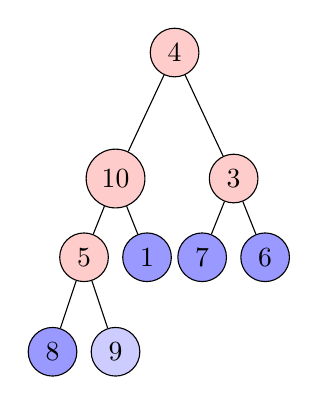
\begin{tikzpicture}[every node/.style={circle,draw,fill=red!20}]
\node {4}
child [level distance=1.6cm, sibling distance=1.5cm]  { node {10}
child[level distance=1cm, sibling distance=0.8cm] { node {5}
child[level distance=1.2cm, sibling distance=0.8cm] { node [fill=blue!40]{8} }
child[level distance=1.2cm, sibling distance=0.8cm] { node[fill=blue!20] {9} }}
child [level distance=1cm, sibling distance=0.8cm]{ node[fill=blue!40] {1} }
}
child[level distance=1.6cm, sibling distance=1.5cm]  { node {3}
child[level distance=1cm, sibling distance=0.8cm] { node[fill=blue!40] {7} }
child[level distance=1cm, sibling distance=0.8cm] { node[fill=blue!40] {6} }
};
\end{tikzpicture}
\end{center}
\textbf{No swaps needed.}
\end{frame}

\begin{frame}{Step 3: Check Node 3 (Valid)}
\begin{center}
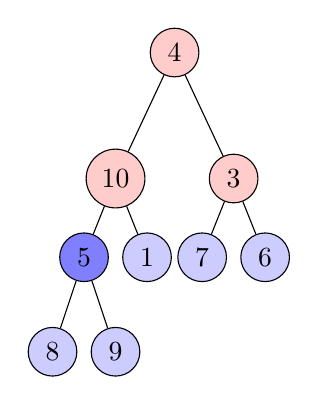
\begin{tikzpicture}[every node/.style={circle,draw,fill=red!20}]
\node {4}
child [level distance=1.6cm, sibling distance=1.5cm]  { node {10}
child[level distance=1cm, sibling distance=0.8cm] { node[fill=blue!50] {5}
child[level distance=1.2cm, sibling distance=0.8cm] { node [fill=blue!20]{8} }
child[level distance=1.2cm, sibling distance=0.8cm] { node[fill=blue!20] {9} }}
child [level distance=1cm, sibling distance=0.8cm]{ node[fill=blue!20] {1} }
}
child[level distance=1.6cm, sibling distance=1.5cm]  { node {3}
child[level distance=1cm, sibling distance=0.8cm] { node[fill=blue!20] {7} }
child[level distance=1cm, sibling distance=0.8cm] { node[fill=blue!20] {6} }
};
\end{tikzpicture}
\end{center}
\textbf{No swaps needed.}
\end{frame}

\begin{frame}{Step 4: Check Node 2 (Valid)}
\begin{center}
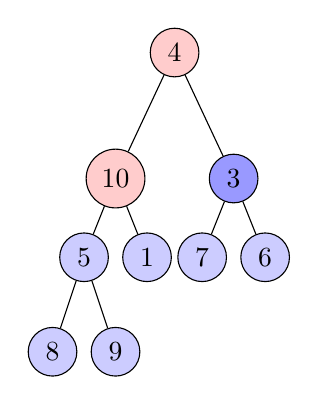
\begin{tikzpicture}[every node/.style={circle,draw,fill=red!20}]
\node {4}
child [level distance=1.6cm, sibling distance=1.5cm]  { node {10}
child[level distance=1cm, sibling distance=0.8cm] { node[fill=blue!20] {5}
child[level distance=1.2cm, sibling distance=0.8cm] { node [fill=blue!20]{8} }
child[level distance=1.2cm, sibling distance=0.8cm] { node[fill=blue!20] {9} }}
child [level distance=1cm, sibling distance=0.8cm]{ node[fill=blue!20] {1} }
}
child[level distance=1.6cm, sibling distance=1.5cm]  { node[fill=blue!40] {3}
child[level distance=1cm, sibling distance=0.8cm] { node[fill=blue!20] {7} }
child[level distance=1cm, sibling distance=0.8cm] { node[fill=blue!20] {6} }
};
\end{tikzpicture}
\end{center}
\textbf{No swaps needed.}
\end{frame}

\begin{frame}{Step 5: Check Node 1 (InValid)}
\begin{center}
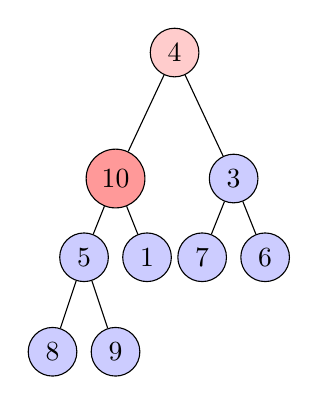
\begin{tikzpicture}[every node/.style={circle,draw,fill=red!20}]
\node {4}
child [level distance=1.6cm, sibling distance=1.5cm]  { node[fill=red!40] {10}
child[level distance=1cm, sibling distance=0.8cm] { node[fill=blue!20] {5}
child[level distance=1.2cm, sibling distance=0.8cm] { node [fill=blue!20]{8} }
child[level distance=1.2cm, sibling distance=0.8cm] { node[fill=blue!20] {9} }}
child [level distance=1cm, sibling distance=0.8cm]{ node[fill=blue!20] {1} }
}
child[level distance=1.6cm, sibling distance=1.5cm]  { node[fill=blue!20] {3}
child[level distance=1cm, sibling distance=0.8cm] { node[fill=blue!20] {7} }
child[level distance=1cm, sibling distance=0.8cm] { node[fill=blue!20] {6} }
};
\end{tikzpicture}
\end{center}
\textbf{swap(currentNode, MIN([leftChild],[rightChild])).}
\end{frame}


\begin{frame}{Step 6: swap(node[1],node[4])}
\begin{center}
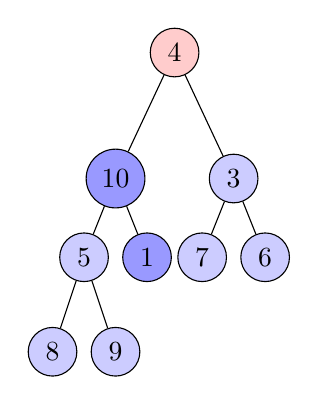
\begin{tikzpicture}[every node/.style={circle,draw,fill=red!20}]
\node {4}
child [level distance=1.6cm, sibling distance=1.5cm]  { node[fill=blue!40] {10}
child[level distance=1cm, sibling distance=0.8cm] { node[fill=blue!20] {5}
child[level distance=1.2cm, sibling distance=0.8cm] { node[fill=blue!20]{8} }
child[level distance=1.2cm, sibling distance=0.8cm] { node[fill=blue!20] {9} }}
child [level distance=1cm, sibling distance=0.8cm]{ node[fill=blue!40] {1} }
}
child[level distance=1.6cm, sibling distance=1.5cm]  { node[fill=blue!20] {3}
child[level distance=1cm, sibling distance=0.8cm] { node[fill=blue!20] {7} }
child[level distance=1cm, sibling distance=0.8cm] { node[fill=blue!20] {6} }
};
\end{tikzpicture}
\end{center}
\textbf{swap(currentNode, MIN([leftChild],[rightChild])).}
\end{frame}

\begin{frame}{Step 6: swap(node[1],node[4])}
\begin{center}
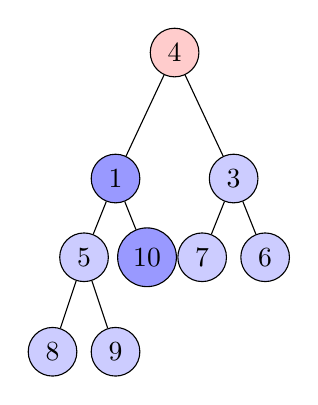
\begin{tikzpicture}[every node/.style={circle,draw,fill=red!20}]
\node {4}
child [level distance=1.6cm, sibling distance=1.5cm]  { node[fill=blue!40] {1}
child[level distance=1cm, sibling distance=0.8cm] { node[fill=blue!20] {5}
child[level distance=1.2cm, sibling distance=0.8cm] { node[fill=blue!20]{8} }
child[level distance=1.2cm, sibling distance=0.8cm] { node[fill=blue!20] {9} }}
child [level distance=1cm, sibling distance=0.8cm]{ node[fill=blue!40] {10} }
}
child[level distance=1.6cm, sibling distance=1.5cm]  { node[fill=blue!20] {3}
child[level distance=1cm, sibling distance=0.8cm] { node[fill=blue!20] {7} }
child[level distance=1cm, sibling distance=0.8cm] { node[fill=blue!20] {6} }
};
\end{tikzpicture}
\end{center}
\textbf{swap(currentNode, MIN([leftChild],[rightChild])).}
\end{frame}

\begin{frame}{Step 7: Check Node 0 (InValid)}
\begin{center}
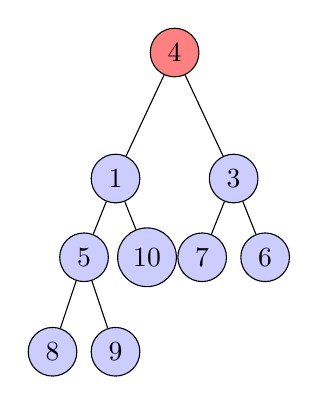
\begin{tikzpicture}[every node/.style={circle,draw,fill=red!20}]
\node[fill=red!50] {4}
child [level distance=1.6cm, sibling distance=1.5cm]  { node[fill=blue!20] {1}
child[level distance=1cm, sibling distance=0.8cm] { node[fill=blue!20] {5}
child[level distance=1.2cm, sibling distance=0.8cm] { node [fill=blue!20]{8} }
child[level distance=1.2cm, sibling distance=0.8cm] { node[fill=blue!20] {9} }}
child [level distance=1cm, sibling distance=0.8cm]{ node[fill=blue!20] {10} }
}
child[level distance=1.6cm, sibling distance=1.5cm]  { node[fill=blue!20] {3}
child[level distance=1cm, sibling distance=0.8cm] { node[fill=blue!20] {7} }
child[level distance=1cm, sibling distance=0.8cm] { node[fill=blue!20] {6} }
};
\end{tikzpicture}
\end{center}
\textbf{swap(currentNode, MIN([leftChild],[rightChild])).}
\end{frame}

\begin{frame}{Step 8: swap(node[0],[1])}
\begin{center}
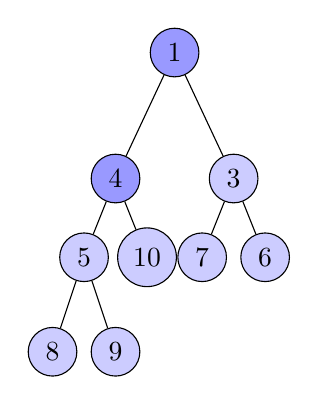
\begin{tikzpicture}[every node/.style={circle,draw,fill=red!20}]
\node[fill=blue!40] {1}
child [level distance=1.6cm, sibling distance=1.5cm]  { node[fill=blue!40] {4}
child[level distance=1cm, sibling distance=0.8cm] { node[fill=blue!20] {5}
child[level distance=1.2cm, sibling distance=0.8cm] { node [fill=blue!20]{8} }
child[level distance=1.2cm, sibling distance=0.8cm] { node[fill=blue!20] {9} }}
child [level distance=1cm, sibling distance=0.8cm]{ node[fill=blue!20] {10} }
}
child[level distance=1.6cm, sibling distance=1.5cm]  { node[fill=blue!20] {3}
child[level distance=1cm, sibling distance=0.8cm] { node[fill=blue!20] {7} }
child[level distance=1cm, sibling distance=0.8cm] { node[fill=blue!20] {6} }
};
\end{tikzpicture}
\end{center}
\textbf{Recursively apply heapify on node[1]]}
\end{frame}

\begin{frame}{Step 9: Heapify}
\begin{center}
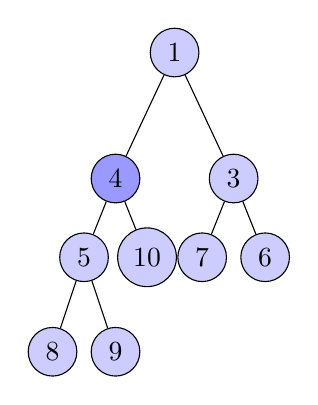
\begin{tikzpicture}[every node/.style={circle,draw,fill=red!20}]
\node[fill=blue!20] {1}
child [level distance=1.6cm, sibling distance=1.5cm]  { node[fill=blue!40] {4}
child[level distance=1cm, sibling distance=0.8cm] { node[fill=blue!20] {5}
child[level distance=1.2cm, sibling distance=0.8cm] { node [fill=blue!20]{8} }
child[level distance=1.2cm, sibling distance=0.8cm] { node[fill=blue!20] {9} }}
child [level distance=1cm, sibling distance=0.8cm]{ node[fill=blue!20] {10} }
}
child[level distance=1.6cm, sibling distance=1.5cm]  { node[fill=blue!20] {3}
child[level distance=1cm, sibling distance=0.8cm] { node[fill=blue!20] {7} }
child[level distance=1cm, sibling distance=0.8cm] { node[fill=blue!20] {6} }
};
\end{tikzpicture}
\end{center}
\textbf{No swap needed.}
\end{frame}

\begin{frame}{Final Heap}
\begin{center}
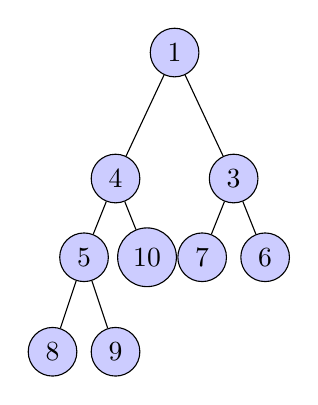
\begin{tikzpicture}[every node/.style={circle,draw,fill=red!20}]
\node[fill=blue!20] {1}
child [level distance=1.6cm, sibling distance=1.5cm]  { node[fill=blue!20] {4}
child[level distance=1cm, sibling distance=0.8cm] { node[fill=blue!20] {5}
child[level distance=1.2cm, sibling distance=0.8cm] { node [fill=blue!20]{8} }
child[level distance=1.2cm, sibling distance=0.8cm] { node[fill=blue!20] {9} }}
child [level distance=1cm, sibling distance=0.8cm]{ node[fill=blue!20] {10} }
}
child[level distance=1.6cm, sibling distance=1.5cm]  { node[fill=blue!20] {3}
child[level distance=1cm, sibling distance=0.8cm] { node[fill=blue!20] {7} }
child[level distance=1cm, sibling distance=0.8cm] { node[fill=blue!20] {6} }
};
\end{tikzpicture}
\end{center}
\end{frame}

\begin{frame}{What Happens at Each Step?}
\textbf{Heapify Explanation:}
\begin{itemize}
\item Start from node $i$.
\item Compare with left-hand([2$i$+1]) and right-hand([2$i$+2]) children.
\item If a child is smaller, swap it with the parent.
\item Recursively apply heapify.
\end{itemize}
\end{frame}

\begin{frame}{HomeWork:}
\begin{center}
    \textbf{Figure out: How long this would take?}
\end{center}
\end{frame}

\begin{frame}{Thank You!}
\begin{center}
    \textbf{Thank you!}
\end{center}
\end{frame}